\chapter[Introducción]{Introducción}
\label{ch:intro}

\section{Motivación}
Los sensores, durante muchos años, han sido herramientas muy útiles en el control de procesos, ya que permiten sensar magnitudes físicas involucradas en los procesos en tiempo real y tener una referencia de lo que está ocurriendo sin necesidad de esperar que finalice un proceso para evaluar el resultado. A medida que los procesos se tornan más complejos, se ha llegado a requerir mayor cantidad de medios para recolectar información. Lo anterior entorpece el desarrollo, debido a la gran cantidad de cables necesarios para alimentar, y extraer información de sensores. Debido a lo anterior, se ha dirigido el  esfuerzo a eliminar estos cableados, lo cual nos lleva un problema: encontrar el equilibrio entre duración de fuente de energía, la cantidad de información capaz de manejar, además de la confiabilidad requerida en este tipo de aplicaciones. Esto ha dado pie al surgimiento de sistemas de redes de sensores inalámbricos ó WSN (Wireless Sensor Network), que se compone por miles, e incluso millones de sensores, que llamaremos nodos, y que son capaces de generar información, procesarla y transmitirla con recursos energéticos limitados. La constante evolución de esta rama de sensores ha abierto un abanico de posibilidades de aplicación; tales como la fabricación de vehículos, domótica, monitorización ambiental, salud, áreas comerciales y militares \cite{crow1997ieee}. En este documento se expone un estudio acerca de las redes TSCH, los principales términos de las redes de sensores, aplicaciones, y los estándares presentes, para luego abordar las redes inalámbricas usando IPv6 bajo el estándar IEEE802.15.4e, y herramientas de simulación.

\section{Fundamentos de redes de sensores}

\subsection{Definición}
Una red de sensores inalámbricos es una red de pequeños dispositivos situados en una determinada localización física, capaces de interactuar con esta red. Las redes de sensores se diseñan de forma específica, y deben distribuirse en un área determinada. Los sensores pueden ser estacionarios o móviles. Los nodos construyen una red Ad-Hoc, donde los dispositivos que la componen son capaces de realizar enrutamiento entre ellos. Para conseguirlo, estos dispositivos se configuran automáticamente sobre una topología determinada, la cual se va actualizando a medida que se modifica su cantidad y localización de modo de permitir un re-enrutamiento dinámico. Existe una variedad de aplicaciones en las que se puede utilizar redes de sensores inalámbricos, entre las que se pueden destacar las siguientes:

\begin{itemize}
    \item Aplicaciones médicas:
    \begin{itemize}
        \item Monitorear signos vitales.
        \item Diagnosticar.
        \item Suministrar medicamentos.
        \item Control ambiental.
        \end{itemize}
    \item Aplicaciones medioambientales:
    \begin{itemize}
        \item Determinar parámetros como luz, temperatura, radiaciones.
        \item Detectar incendios forestales.
        \item Monitorear contaminación.
        \item Censar velocidad y temperatura de vientos.
        \end{itemize}
        
        \newpage
    \item Aplicaciones en maquinaria:
    \begin{itemize}
        \item Medir movimientos y vibraciones.
        \item Censar temperatura, ruidos.
        \item Estimar magnitudes como velocidad, aceleración, dirección, etc.
        \end{itemize}
    \end{itemize}


Para cada aplicación es necesario que los sensores sean capaces de entregar un desempeño confiable. Por ejemplo; en aplicaciones médicas es necesario que sea fiable la transmisión de datos, debe tenerse presente que el monitoreo de signos vitales es crítico para el individuo y no se debe dar espacio a incertidumbres. Caso similar para la aplicación en monitoreo medioambiental, donde se necesita que los sistemas sean capaces de alertar de un eventual incendio lo más pronto posible. Para el caso de aplicaciones en maquinaria, también es necesario tener la información rápidamente para prevenir posibles daños frente a situaciones de sobre exigencia, temperatura o fatiga de materiales.

Cuando se trabaja con estas redes, es necesario identificar qué componentes se necesita utilizar para tener datos precisos y correctos. A continuación se muestran los componentes disponibles para utilizar en una implementación de redes de sensores.




\subsection{Elementos}

\begin{itemize}
    \item Sensores: Existen de diferente naturaleza, su función es capturar información del entorno, y codificarla en formato digital.
    \item Nodo sensor: O también llamados, en algunos países, ``motes'' o procesadores de radio. Su función es tomar los datos del sensor a través de sus entradas de datos, y enviarlos o propagarlos. Este es el conjunto de nodo transmisor y sensor o sensores.
    \item Nodo: Es un sensor, puede o no contener procesador de radio, cuando este es el caso, pasa a ser un nodo sensor.
    \item Puerta de enlace: Punto de conexión entre los nodos, y una red TCP/IP.
    \item Estación base: Etapa o sistema, el cual recibe o recopila los datos. Puede ser un computador, u otro nodo de la red.
\end{itemize}

Los elementos descritos deben ser capaces de interactuar entre sí para intercambiar información. Para lo anterior, es necesario que cada componente utilice un lenguaje estándar para comunicarse entre sí, esto permite plantear el concepto de estándares de comunicación, el cual se explicará a continuación.



\subsection{Estándares}

Al iniciarse el desarrollo de las redes inalámbricas, cada fabricante tenía sus propios métodos y lenguajes para interconectarse con otros dispositivos fabricados por el mismo. Aquello funcionaba muy bien para sus propios dispositivos, pero no así para los distribuidos por otro fabricante. Por otro lado, sus clientes debían estar dispuestos a adquirir solamente equipos de sólo un fabricante fabricante. Esto trajo consigo malas prácticas en cierto modo monopólicas.

Entrando en el año 1997, el Instituto de Ingenieros Eléctricos y Electrónicos (IEEE), tomando características de sistemas de comunicación junto a un grupo de distintos fabricantes de sistemas de telecomunicaciones, generó y estableció un protocolo universal que permitía manufacturar tanto dispositivos de emisión, como de recepción. Estos dispositivos debían poder interactuar con los de otro productor que cumplieran el mismo estándar. Esto dió origen al estándar 802.11. \cite{crow1997ieee}

Conforme pasan los años, los sistemas de telecomunicaciones se hacen más capaces, y las exigencias se incrementan, por lo tanto, los protocolos quedan obsoletos, es por esto que se hace necesario que se actualicen los estándares, agregándoles características, y reemplazando otras. La situación antes descrita da origen a las revisiones, las cuales incluyen mejoras junto al estándar base, y se denominan añadiendo una identificación al protocolo como fue el caso de 802.11a, cuya mejora posteriormente fue agregada por completo al protocolo 802.11, manteniendo este mismo nombre final.

Por lo tanto, hoy en día la tecnología de las redes inalámbricas se basa en estándares que tienen como misión alcanzar un equilibrio entre velocidad de transmisión, cobertura y coste energético por paquete enviado. Para conseguir esto, se han creado protocolos que comandan la interconexión y comunicación entre dispositivos. Cada protocolo define reglas que deben cumplirse fielmente para garantizar el correcto desempeño de una comunicación. 

Este documento se basa en la implementación por parte de la IETF del protocolo IP versión 6 sobre una red “Time slotted channel hopping”, TSCH por sus siglas en inglés, nombrado también bajo estándar IEEE802.15.4e. Una red TSCH es una red capaz de ajustar su canal de comunicación a un espacio de tiempo asignado por un calendarizador, el que puede ser implementado utilizando diferentes algoritmos, los cuales serán abordados en este documento. \cite{dujovne20146tisch}

\subsubsection{Estándares relacionados}

Es necesario destacar que las redes TSCH han sido desarrolladas por distintos organismos, que les han dado una aplicación diferente según el área de la industria. Por un lado, tenemos las redes industriales TSCH WirelessHART, y por el otro, tenemos las redes ISA100.11a. Ambas redes se basan en el estándar IEEE802.15.4, el cual opera en una frecuencia de 2.4 Gigahertz. Ambos son utilizados en una amplia gama de aplicaciones industriales, sobre todo en procedimientos de automatización de procesos, y de plantas de producción.
Ambos estándares son usados como LoWPAN (redes inalámbricas de área personal de baja tasa de transferencia, por sus siglas en inglés). ISA100.11a usa una capa MAC la que es una versión modificada de la capa MAC utilizada por WirelessHART. Ambas utilizan el mismo mecanismo para el transporte de datos desde y hasta la puerta de enlace. Como ambas tecnologías operan en muy baja potencia, la vida de sus baterías es extensa.
Sus radios utilizan DSSS (ampliación de espectro por secuencia directa por sus siglas en inglés) para permitir la coexistencia del mismo espectro de frecuencia sin generar ninguna clase de interferencia entre ellas.

\begin{figure}
\centering
\graphicspath{ {imagenes/} }
\begin{minipage}{.5\textwidth}
  \centering
  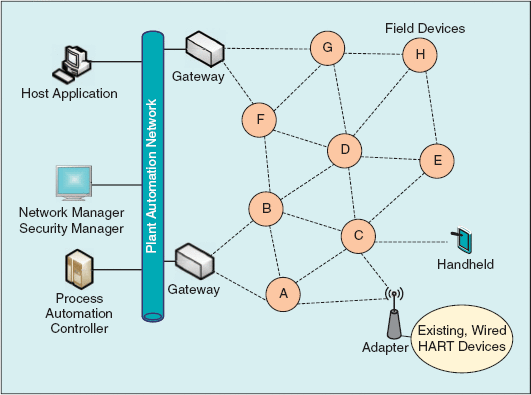
\includegraphics[width=.9\linewidth]{HART.png}
  \captionof{figure}{Imagen de una red WirelessHART}
  \label{HART}
\end{minipage}%
\begin{minipage}{.5\textwidth}
  \centering
  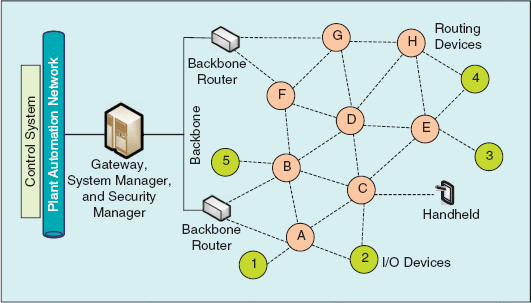
\includegraphics[width=.9\linewidth]{ISA100.png}
  \captionof{figure}{Imagen de una red ISA100.11a}
  \label{ISA100}
\end{minipage}
\end{figure}

Las imágenes \ref{HART}, y \ref{ISA100} muestran las similitudes y diferencias entre estos dos tipos de estándares.\cite{petersen2011wirelesshart}




A pesar que el estándar ha tenido dos revisiones, el de la capa física no ha cambiado, sino que se ha incorporado una nueva capa MAC como complemento al modelo IEEE802.15.4 \cite{RFC7554}, siendo esta capa MAC ahora sincrónica y que asigna recursos por frecuencia y tiempo de manera simultánea. \cite{watteyne2015using}

Cabe mencionar que este stack es utilizado en redes 6LoWPAN, equivalente al stack TCP/IP, pero adaptado a las redes (low powered and lossy networks) LLN por sus siglas en inglés. La imagen a continuación muestra las diferencias entre estos protocolos.

\begin{figure}[h]
\centering
\graphicspath{ {imagenes/} }
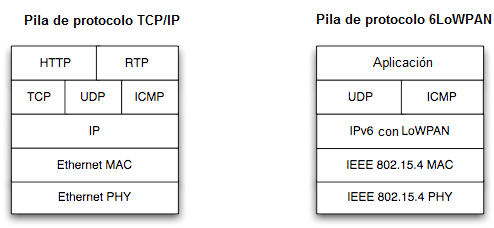
\includegraphics[width=0.9\textwidth]{stack.png}
\caption{Comparación entre stack 6LoWPAN y TCP/IP}
\label{stack}
\end{figure}

Los estándares mencionados son los que se usarán en este estudio, los que están contenidos en el protocolo 6TiSCH, el que se abordará a continuación.




\subsection{6TiSCH: IPv6 sobre redes IEEE802.15.4e TSCH}


Una red TSCH, es una red cuyo calendarizador es quien controla la comunicación, esto implica que el controlador asigna celdas de tiempo/frecuencia entre los nodos vecinos. Asignar múltiples espacios de tiempo a los mismos vecinos aumenta la cantidad de datos que estos nodos pueden intercambiar por segundo y reduce la latencia en la comunicación, pero por otro lado, esto implica que la radio de los nodos deberá estar encendida mas tiempo, aumentando el consumo energético promedio, y reduciendo la vida de su batería. Este documento aborda una perspectiva de la implementación del protocolo IP versión 6 sobre una red TSCH en la que se busca mejorar el desempeño de asignación de celdas de comunicación.

6TiSCH define un nuevo concepto global, el cual se llama ``Matriz de distribución de canal/uso'' (CDU) por sus siglas en inglés con una altura igual a la cantidad de frecuencias disponibles (indexados por una lista de distribución de canales) y un ancho en espacios de tiempo, que corresponde al ``período'' de la operación de calendarización de la red (indexados por una lista de acomodación de espacios, o ``slots'').

La matriz CDU puede ser particionada en trozos, los que llamaremos ``chunk'' por su nombre en inglés, un chunk es conocido globalmente por todos los nodos en la red para dar apoyo en el proceso de apropiación, el cual es una negociación entre nodos dentro de un dominio de interferencias.

Un nodo que se apropia de un chunk decide qué transmisiones van a ocurrir sobre las celdas en el chunk, dentro de su dominio de interferencia. Por último, un chunk representa una asignación de ancho de banda y puede ser visto como la generalización de un canal de transmisión en el dominio de tiempo/frecuencia.

\newpage
\subsubsection{Arquitectura}

6TiSCH está encausado en lograr el poco común hito de entregar una arquitectura que abarca múltiples estándares de diversas áreas dentro de de la IETF. La arquitectura 6TiSCH está actualmente siendo diseñada con el objetivo de proveer altos PDR (Packet Delivery Rate por sus siglas en inglés) y latencia determinista de acuerdo a los protocolos de las redes de sensores inalámbricas industriales, como son ``WirelessHART'', y ``ISA100.11a''. Además, permite implementaciones de monitoreos de gran escala con el fin de cubrir el paradigma de internet industrial.

Con el fin de hacerlo escalable, y manteniendo el ancho de banda, la operación de ``6LoWPAN Neighbor Discovery (ND)'' se realiza dentro de la red, para eliminar la necesidad de realizar ``multicast'' e inundaciones, inherentes a la operación de la búsqueda de vecinos (ND) clásica de IPv6.

La experiencia de una WSN industrial da soporte a una aproximación centralizada, permitiendo un control total, y una optimización de la operación de la red desde un motor central de cómputo, con una “vista de dios”, la cual es llamada Administrador de red (Network manager en inglés), o Administrador de sistema, y que corresponde al Elemento de Cálculo del camino(PCE) en inglés, de la IETF. PCE considera todos los flujos y toda la capacidad de la red, calculando el grupo de pistas ``punto a punto'' (end-to-end) óptimo.

La arquitectura 6TiSCH debe cubrir todos los componentes tales como como seguridad y administración. Estos componentes afectan a todos los aspectos de las operaciones de la unidad, y cada una de las variadas técnicas que existen pueden ser relevantes para 6TiSCH. Sin embargo las limitaciones en memoria, CPU, ancho de banda, y latencia permiten implementar soluciones, pero son poco prácticas, y la necesidad de una red de alta escalabilidad y bajo mantenimiento motiva la implementación de sistemas autónomos.

6TiSCH apunta a la reutilización de código para distintos componentes, para así evitar cualquier duplicación funcional. Es por esto que se considera el manejo sobre Protocolo de Aplicación Restringida ``Constrained Application Protocol'' (CoAP), para reusar el código que servirá para registrar la información del sensor, y la Seguridad del Datagrama de la Capa de transporte (DTLS).

\subsection{Mecanismos de calendarización}

Realizar una calendarización en una red TSCH requiere de mecanismos que conforman una política para operar este calendarizador en la red.

La política está a cargo de determinar qué espacio de tiempo está asignado, y a cuál nodo. La calendarización puede ser vista como un problema de optimización, donde los espacios de tiempos son asignados para parearse con los nodos vecinos conectados para satisfacer los requerimientos a nivel de capa de aplicación. Estos requerimientos pueden ser expresados como métricas que el algoritmo debe optimizar, contemplando colisiones, consumo de energía, latencia, o la combinación de estos.

6TiSCH no necesariamente asume la calendarización como una sola entidad, puede ser distribuida, o centralizada. La ``entidad'' que realiza la calendarización se basa en mecanismos utilizados para realizar calendarizaciones, como por ejemplo el formato de paquetes para acceder al calendario de TSCH.

Hasta principios del año dos mil dieciséis existían cuatro tipos de mecanismos de calendarización en uso: Static Scheduling, Neighbor-to-neighbor Scheduling, Remote Monitoring and Schedule Management, y Hop-by-hop Scheduling \cite{ietf-6tisch-architecture-10}. Recientemente, tras la publicación de \cite{muraoka2016simple} el veinticinco de Mayo, se añade un quinto método de calendarizador, su nombre es Distributed scheduling o Calendarización distribuida.

\subsubsection{Static Scheduling}

El Calendarizado estático, o Static Scheduling hace referencia a la operación mínima de 6TiSCH, por el cual un programa estático configurado para toda la red utiliza el sistema aloha, pero ajustado a los espacios de tiempo en el cual el nodo puede transmitir, este protocolo recibe el nombre de S-Aloha, acrónimo de Slotted Aloha. El calendarizador es distribuido a travéz de todos los métodos nativos que podemos encontrar en una capa MAC TSCH. Esta operación aprovecha el protocolo RPL (Routing Protocol for Low-Power and Lossy Networks con sus siglas en inglés) para mantener un gráfico sin retornos del enrutamiento y la distribución de tiempo.


\subsubsection{Neighbor-to-neighbor Scheduling}

El calendarizador vecino a vecino utiliza adaptación dinámica del ancho de banda de los enlaces que se utilizan para el tráfico IPv6 entre los enrutadores adyacentes. Las funciones como SF0 influencian la operación de la subcapa 6top para añadir o eliminar celdas en un calendarizador vecino, usando el protocolo 6top para negociar con los recursos de la capa MAC.

\subsubsection{Remote Monitoring and Schedule Management}

El monitoreo remoto, y manejo de calendarizador se hace referencia al cálculo central de un calendarizador, y la capacidad de reenviar una trama en base a la celda de llegada. En este mecanismo, la sección correspondiente al calendarizador de la unidad, así como también los otros recursos del dispositivo son gestionados por una unidad abstracta de manejo de red, la cual puede cooperar con el elemento de cómputo de ruta (PCE por sus siglas en inglés) con el fin de reducir la interacción con el, y por lo tanto, evitar la sobrecarga del dispositivo.

\subsubsection{Hop-by-hop Scheduling}

El calendarizador salto a salto permite que un nodo pueda reservar una unidad de asignación varias unidades por delante, utilizando celdas flexibles en cada nodo intermedio, esto forma una pista de celdas flexibles. La subcapa 6top de cada nodo es la responsable de controlar las celdas flexibles, y reubicarlas cuando sea necesario. Aún no esta definido el protocolo para activar el calendarizador salto a salto.


\subsubsection{Distributed scheduling}

El calendarizador distribuido es otra alternativa recientemente implementada, la que consiste en que cada nodo utiliza 6top para negociar, añadiendo un número de celdas correspondientes a los requerimientos de ancho de banda. El nodo construye un requerimiento para añadir, el cual incluye una lista aleatoriamente seleccionada de celdas candidatas. Esta lista es enviada al nodo vecino, el que revisa en su lista cual de estas celdas seleccionadas no esta siendo actualmente utilizada, para seleccionar una de estas aleatoriamente y enviarla como respuesta al nodo anterior. Por lo tanto, cada nodo vecino negocia el uso de espacios de tiempo con los otros, sin requerir la intervención de una entidad central. 6TiSCH está estandarizando el formato de los paquetes intercambiados entre los nodos vecinos para conducir la negociación. Aún así existen colisiones, pero la capa 6top es la encargada de lidiar con esta situación para establecer una conexión confiable.
\cite{muraoka2016simple}

